\providecommand{\main}{..}
\documentclass[\main/main.tex]{subfiles}
\begin{document}
\clearpage
\section{CpGobsExp}
\subsection{Metric sample distribution}
The data points seem to follow a \textbf{Beta} distribution with the following parameters:

\begin{align*}
  \alpha   = 7.6689746880295795          & \qquad  \beta = 6778383.524935903       \\
  \text{location} = -0.09826818916997124 & \qquad \text{scale} = 306278.3184506849
\end{align*}

\begin{figure}
  \includegraphics[width=\textwidth]{metrics_statistics/CpGobsExp}
  \caption{Sampling distribution of metric CpGobsExp}
\end{figure}
\subsection{Metric values}
\begin{figure}
  \includegraphics[width=\textwidth]{metrics_plot/CpGobsExp}
  \caption{Values of metric CpGobsExp}
\end{figure}

\clearpage
\section{CpGperCpG}
\subsection{Metric sample distribution}
The data points seem to follow a \textbf{Beta} distribution with the following parameters:

\begin{align*}
  \alpha   = 6.402175341881067           & \qquad  \beta = 97129163.31117742      \\
  \text{location} = -0.05698922703576313 & \qquad \text{scale} = 4337764.42876015
\end{align*}
\begin{figure}
  \includegraphics[width=\textwidth]{metrics_statistics/CpGperCpG}
  \caption{Sampling distribution of metric CpGperCpG}
\end{figure}
\subsection{Metric values}
\begin{figure}
  \includegraphics[width=\textwidth]{metrics_plot/CpGperCpG}
  \caption{Values of metric CpGperCpG}
\end{figure}

\clearpage
\section{CpGperGC}
\subsection{Metric sample distribution}
The data points seem to follow a \textbf{Gaussian} distribution with the following parameters:

\begin{align*}
  \mean{X} = 0.4602356242601636 & \qquad \Var{X} = 0.15949294643574352
\end{align*}
\begin{figure}
  \includegraphics[width=\textwidth]{metrics_statistics/CpGperGC}
  \caption{Sampling distribution of metric CpGperGC}
\end{figure}
\subsection{Metric values}
\begin{figure}
  \includegraphics[width=\textwidth]{metrics_plot/CpGperGC}
  \caption{Values of metric CpGperGC}
\end{figure}

\clearpage
\section{DGVCount}
\subsection{Metric sample distribution}
The data points seem to follow a \textbf{Gamma} distribution with the following parameters:
\begin{align*}
  \alpha   = 0.20940038672579409    \qquad  \text{location} = -1.1962983066939984e-30 \qquad \text{scale} = 1.2347090894162929
\end{align*}
\begin{figure}
  \includegraphics[width=\textwidth]{metrics_statistics/DGVCount}
  \caption{Sampling distribution of metric DGVCount}
\end{figure}
\subsection{Metric values}
\begin{figure}
  \includegraphics[width=\textwidth]{metrics_plot/DGVCount}
  \caption{Values of metric DGVCount}
\end{figure}

\clearpage
\section{DnaseClusteredHyp}
\subsection{Metric sample distribution}
The data points seem to follow a \textbf{Gamma} distribution with the following parameters:
\begin{align*}
  \alpha   = 0.4176887081406805    \qquad  \text{location} = -3.362626207862299e-29 \qquad \text{scale} = 0.3676310948709975
\end{align*}
\begin{figure}
  \includegraphics[width=\textwidth]{metrics_statistics/DnaseClusteredHyp}
  \caption{Sampling distribution of metric DnaseClusteredHyp}
\end{figure}
\subsection{Metric values}
\begin{figure}
  \includegraphics[width=\textwidth]{metrics_plot/DnaseClusteredHyp}
  \caption{Values of metric DnaseClusteredHyp}
\end{figure}

\clearpage
\section{DnaseClusteredScore}
\subsection{Metric sample distribution}
The data points seem to follow \textbf{slightly} a \textbf{Beta} distribution with the following parameters:
\begin{align*}
  \alpha   = 0.2709657632937803          & \qquad  \beta = 0.44530002562349713      \\
  \text{location} = -0.09309893086089688 & \qquad \text{scale} = 1.0930989308608972
\end{align*}

\begin{figure}
  \includegraphics[width=\textwidth]{metrics_statistics/DnaseClusteredScore}
  \caption{Sampling distribution of metric DnaseClusteredScore}
\end{figure}
\subsection{Metric values}
\begin{figure}
  \includegraphics[width=\textwidth]{metrics_plot/DnaseClusteredScore}
  \caption{Values of metric DnaseClusteredScore}
\end{figure}

\clearpage
\section{EncH3K27Ac}
\subsection{Metric sample distribution}
The data points seem to follow a family of \textbf{Gamma} distributions (a speculation for this distribution could be the different groups from which the data are extracted), we will approximate them to one with a linear combination of the parameters:
\begin{align*}
  \alpha   = 0.0004042086221537893    \qquad  \text{location} = -2.859398162696207e-24 \qquad \text{scale} = 0.03076944787133299
\end{align*}
\begin{figure}
  \includegraphics[width=\textwidth]{metrics_statistics/EncH3K27Ac}
  \caption{Sampling distribution of metric EncH3K27Ac}
\end{figure}
\subsection{Metric values}
\begin{figure}
  \includegraphics[width=\textwidth]{metrics_plot/EncH3K27Ac}
  \caption{Values of metric EncH3K27Ac}
\end{figure}

\clearpage
\section{EncH3K4Me1}
\subsection{Metric sample distribution}
The data points seem to follow a family of \textbf{Gamma} distributions (a speculation for this distribution could be the different groups from which the data are extracted), we will approximate them to one with a linear combination of the parameters:
\begin{align*}
  \alpha   = 0.22566387737236238    \qquad  \text{location} = -6.619765504581537e-27 \qquad \text{scale} = 1.396157055181753
\end{align*}
\begin{figure}
  \includegraphics[width=\textwidth]{metrics_statistics/EncH3K4Me1}
  \caption{Sampling distribution of metric EncH3K4Me1}
\end{figure}
\subsection{Metric values}
\begin{figure}
  \includegraphics[width=\textwidth]{metrics_plot/EncH3K4Me1}
  \caption{Values of metric EncH3K4Me1}
\end{figure}

\clearpage
\section{EncH3K4Me3}
\subsection{Metric sample distribution}
The data points seem to follow a family of \textbf{Gamma} distributions (a speculation for this distribution could be the different groups from which the data are extracted), we will approximate them to one with a linear combination of the parameters:
\begin{align*}
  \alpha   = 0.007502428717446465    \qquad  \text{location} = -3.469650119186857e-25 \qquad \text{scale} = 0.04125297431971783
\end{align*}
\begin{figure}
  \includegraphics[width=\textwidth]{metrics_statistics/EncH3K4Me3}
  \caption{Sampling distribution of metric EncH3K4Me3}
\end{figure}
\subsection{Metric values}
\begin{figure}
  \includegraphics[width=\textwidth]{metrics_plot/EncH3K4Me3}
  \caption{Values of metric EncH3K4Me3}
\end{figure}

\clearpage
\section{GCContent}
\subsection{Metric sample distribution}
The data points seem to be a combination of two \textbf{Gaussian} distributions. This will be approximated to one with the following parameters:

\begin{align*}
  \mean{X} = 0.4482813176478024 & \qquad \Var{X} = 0.1097424869360011
\end{align*}
\begin{figure}
  \includegraphics[width=\textwidth]{metrics_statistics/GCContent}
  \caption{Sampling distribution of metric GCContent}
\end{figure}
\subsection{Metric values}
\begin{figure}
  \includegraphics[width=\textwidth]{metrics_plot/GCContent}
  \caption{Values of metric GCContent}
\end{figure}

\clearpage
\section{GerpRS}
\subsection{Metric sample distribution}
The data points seem to follow a family of \textbf{Gamma} distributions (a speculation for this distribution could be the different groups from which the data are extracted), we will approximate them to one with a linear combination of the parameters:
\begin{align*}
  \alpha   = 0.8688332877203315    \qquad  \text{location} = -1.7081810436826354e-28 \qquad \text{scale} = 0.11512094125204281
\end{align*}
\begin{figure}
  \includegraphics[width=\textwidth]{metrics_statistics/GerpRS}
  \caption{Sampling distribution of metric GerpRS}
\end{figure}
\subsection{Metric values}
\begin{figure}
  \includegraphics[width=\textwidth]{metrics_plot/GerpRS}
  \caption{Values of metric GerpRS}
\end{figure}

\clearpage
\section{GerpRSpv}
\subsection{Metric sample distribution}
The data points seem to follow a family of \textbf{Gamma} distributions (a speculation for this distribution could be the different groups from which the data are extracted), we will approximate them to one with a linear combination of the parameters:
\begin{align*}
  \alpha   = 0.5165290213220888    \qquad  \text{location} = -6.952792177974854e-30 \qquad \text{scale} = 0.2530358950266992
\end{align*}
\begin{figure}
  \includegraphics[width=\textwidth]{metrics_statistics/GerpRSpv}
  \caption{Sampling distribution of metric GerpRSpv}
\end{figure}
\subsection{Metric values}
\begin{figure}
  \includegraphics[width=\textwidth]{metrics_plot/GerpRSpv}
  \caption{Values of metric GerpRSpv}
\end{figure}

\clearpage
\section{ISCApath}
\subsection{Metric sample distribution}
The data points seem to follow a \textbf{Gamma} distribution with the following parameters:
\begin{align*}
  \alpha   = 0.08318618903703257    \qquad  \text{location} = -1.9358902729364646e-30 \qquad \text{scale} = 1.2606790181148981
\end{align*}
\begin{figure}
  \includegraphics[width=\textwidth]{metrics_statistics/ISCApath}
  \caption{Sampling distribution of metric ISCApath}
\end{figure}
\subsection{Metric values}
\begin{figure}
  \includegraphics[width=\textwidth]{metrics_plot/ISCApath}
  \caption{Values of metric ISCApath}
\end{figure}

\clearpage
\section{commonVar}
\subsection{Metric sample distribution}
The data points seem to follow an \textbf{Exponential Weibull} distribution with the following parameters:

\begin{align*}
  \alpha   = 5.038707296051438            & \qquad  \beta = 1.0160276119461702         \\
  \text{location} = -0.012528678364149837 & \qquad \text{scale} = 0.025052745155722922
\end{align*}
\begin{figure}
  \includegraphics[width=\textwidth]{metrics_statistics/commonVar}
  \caption{Sampling distribution of metric commonVar}
\end{figure}
\subsection{Metric values}
\begin{figure}
  \includegraphics[width=\textwidth]{metrics_plot/commonVar}
  \caption{Values of metric commonVar}
\end{figure}

\clearpage
\section{dbVARCount}
\subsection{Metric sample distribution}
The data points seem to follow a \textbf{Gamma} distribution with the following parameters:
\begin{align*}
  \alpha   = 0.20940038672579409    \qquad  \text{location} = -1.1962983066939984e-30 \qquad \text{scale} = 1.2347090894162929
\end{align*}
\begin{figure}
  \includegraphics[width=\textwidth]{metrics_statistics/dbVARCount}
  \caption{Sampling distribution of metric dbVARCount}
\end{figure}
\subsection{Metric values}
\begin{figure}
  \includegraphics[width=\textwidth]{metrics_plot/dbVARCount}
  \caption{Values of metric dbVARCount}
\end{figure}

\clearpage
\section{fantom5Perm}
\subsection{Metric sample distribution}
The data points seem to follow a \textbf{Gamma} distribution with the following parameters:
\begin{align*}
  \alpha   = 0.06895533706017208    \qquad  \text{location} = -3.220296247423778e-30 \qquad \text{scale} = 1.2605014923175824
\end{align*}
\begin{figure}
  \includegraphics[width=\textwidth]{metrics_statistics/fantom5Perm}
  \caption{Sampling distribution of metric fantom5Perm}
\end{figure}
\subsection{Metric values}
\begin{figure}
  \includegraphics[width=\textwidth]{metrics_plot/fantom5Perm}
  \caption{Values of metric fantom5Perm}
\end{figure}

\clearpage
\section{fantom5Robust}
\subsection{Metric sample distribution}
The data points seem to follow a \textbf{Gamma} distribution with the following parameters:
\begin{align*}
  \alpha   = 0.08983952110680529    \qquad  \text{location} = -3.220296247423778e-30 \qquad \text{scale} = 1.2605014923175824
\end{align*}
\begin{figure}
  \includegraphics[width=\textwidth]{metrics_statistics/fantom5Robust}
  \caption{Sampling distribution of metric fantom5Robust}
\end{figure}
\subsection{Metric values}
\begin{figure}
  \includegraphics[width=\textwidth]{metrics_plot/fantom5Robust}
  \caption{Values of metric fantom5Robust}
\end{figure}

\clearpage
\section{fracRareCommon}
\subsection{Metric sample distribution}
The data points seem to follow an \textbf{Beta} distribution with the following parameters:

\begin{align*}
  \alpha   = 2772.739504773501         & \qquad  \beta = 14.986077009876375      \\
  \text{location} = -69.93503912437342 & \qquad \text{scale} = 71.09741090721741
\end{align*}
\begin{figure}
  \includegraphics[width=\textwidth]{metrics_statistics/fracRareCommon}
  \caption{Sampling distribution of metric fracRareCommon}
\end{figure}
\subsection{Metric values}
\begin{figure}
  \includegraphics[width=\textwidth]{metrics_plot/fracRareCommon}
  \caption{Values of metric fracRareCommon}
\end{figure}

\clearpage
\section{mamPhastCons46way}
\subsection{Metric sample distribution}
The data points seem to follow a \textbf{Gamma} distribution with the following parameters:
\begin{align*}
  \alpha   = 0.3215099801387991    \qquad  \text{location} = -6.260887365023215e-31 \qquad \text{scale} = 0.45230902834164866
\end{align*}
\begin{figure}
  \includegraphics[width=\textwidth]{metrics_statistics/mamPhastCons46way}
  \caption{Sampling distribution of metric mamPhastCons46way}
\end{figure}
\subsection{Metric values}
\begin{figure}
  \includegraphics[width=\textwidth]{metrics_plot/mamPhastCons46way}
  \caption{Values of metric mamPhastCons46way}
\end{figure}

\clearpage
\section{mamPhyloP46way}
\subsection{Metric sample distribution}
The data points seem to follow a \textbf{Gaussian} distribution with the following parameters:

\begin{align*}
  \mean{X} = 0.7032457913828309 & \qquad \Var{X} = 0.07627203289198752
\end{align*}
\begin{figure}
  \includegraphics[width=\textwidth]{metrics_statistics/mamPhyloP46way}
  \caption{Sampling distribution of metric mamPhyloP46way}
\end{figure}
\subsection{Metric values}
\begin{figure}
  \includegraphics[width=\textwidth]{metrics_plot/mamPhyloP46way}
  \caption{Values of metric mamPhyloP46way}
\end{figure}

\clearpage
\section{numTFBSConserved}
\subsection{Metric sample distribution}
The data points seem to follow a \textbf{exponential} distribution with the following parameters:

\begin{align*}
  \mean{X} = -4.600037873301623e-12 & \qquad \Var{X} = 0.033419421646804975
\end{align*}
\begin{figure}
  \includegraphics[width=\textwidth]{metrics_statistics/numTFBSConserved}
  \caption{Sampling distribution of metric numTFBSConserved}
\end{figure}
\subsection{Metric values}
\begin{figure}
  \includegraphics[width=\textwidth]{metrics_plot/numTFBSConserved}
  \caption{Values of metric numTFBSConserved}
\end{figure}

\clearpage
\section{priPhastCons46way}
\subsection{Metric sample distribution}
The data points seem to follow a \textbf{Gamma} distribution with the following parameters:
\begin{align*}
  \alpha   = 0.2836383862597563    \qquad  \text{location} = -1.8643137904859329e-31 \qquad \text{scale} = 0.37399746075497264
\end{align*}
\begin{figure}
  \includegraphics[width=\textwidth]{metrics_statistics/priPhastCons46way}
  \caption{Sampling distribution of metric priPhastCons46way}
\end{figure}
\subsection{Metric values}
\begin{figure}
  \includegraphics[width=\textwidth]{metrics_plot/priPhastCons46way}
  \caption{Values of metric priPhastCons46way}
\end{figure}

\clearpage
\section{priPhyloP46way}
\subsection{Metric sample distribution}
The data points seem to follow an \textbf{Beta} distribution with the following parameters:

\begin{align*}
  \alpha   = 2095270.7440875275         & \qquad  \beta = 4.199025269606416        \\
  \text{location} = -103376.03746996864 & \qquad \text{scale} = 103377.03863437689
\end{align*}
\begin{figure}
  \includegraphics[width=\textwidth]{metrics_statistics/priPhyloP46way}
  \caption{Sampling distribution of metric priPhyloP46way}
\end{figure}
\subsection{Metric values}
\begin{figure}
  \includegraphics[width=\textwidth]{metrics_plot/priPhyloP46way}
  \caption{Values of metric priPhyloP46way}
\end{figure}

\clearpage
\section{rareVar}
\subsection{Metric sample distribution}
The data points seem to follow an \textbf{Beta} distribution with the following parameters:

\begin{align*}
  \alpha   = 14.148202647100376           & \qquad  \beta = 7669045.025220526        \\
  \text{location} = -0.008523116473417407 & \qquad \text{scale} = 28973.953544984728
\end{align*}
\begin{figure}
  \includegraphics[width=\textwidth]{metrics_statistics/rareVar}
  \caption{Sampling distribution of metric rareVar}
\end{figure}
\subsection{Metric values}
\begin{figure}
  \includegraphics[width=\textwidth]{metrics_plot/rareVar}
  \caption{Values of metric rareVar}
\end{figure}

\clearpage
\section{verPhastCons46way}
\subsection{Metric sample distribution}
The data points seem to follow a \textbf{Gamma} distribution with the following parameters:
\begin{align*}
  \alpha   = 0.4378982063415524    \qquad  \text{location} = -2.5307968883256733e-31 \qquad \text{scale} = 0.43138079305533483
\end{align*}
\begin{figure}
  \includegraphics[width=\textwidth]{metrics_statistics/verPhastCons46way}
  \caption{Sampling distribution of metric verPhastCons46way}
\end{figure}
\subsection{Metric values}
\begin{figure}
  \includegraphics[width=\textwidth]{metrics_plot/verPhastCons46way}
  \caption{Values of metric verPhastCons46way}
\end{figure}

\clearpage
\section{verPhyloP46way}
\subsection{Metric sample distribution}
The data points seem to follow a \textbf{Gaussian} distribution with the following parameters:

\begin{align*}
  \mean{X} = 0.5723779382558164 & \qquad \Var{X} = 0.0662715947139185
\end{align*}
\begin{figure}
  \includegraphics[width=\textwidth]{metrics_statistics/verPhyloP46way}
  \caption{Sampling distribution of metric verPhyloP46way}
\end{figure}
\subsection{Metric values}
\begin{figure}
  \includegraphics[width=\textwidth]{metrics_plot/verPhyloP46way}
  \caption{Values of metric verPhyloP46way}
\end{figure}

\end{document}
